\chapter{What is Combinatorics?}
\section{Introduction}
This course aims to delve into the study of discrete mathematical structures, a field which traces its roots back to the 1700s with the work of Leonhard Euler and has gained much attention between the 1960s and 1970s with the advent of computer science. Notably, Euler answered the following question posed by Philip Naude in the year 1741: “In how many ways can the number $50$ be written as a sum of seven different positive integers?”. We shall understand the outline of Euler’s solution to the problem later in this course. A few important personalities (some of whose work we will study eventually) in the subject include Gian Carlo Rota, Donald Knuth, Richard Stanley, Srinivasa Ramanujan, and Pinagala. 

Combinatorics is the science of patterns and arrangements. More concretely, it deals with the study of the existence and the number of arrangements possible for a given mathematical structure. We start our discussion with a few motivating questions which will make our statement clearer.

\begin{question}
	In how many ways can you arrange the elements of the set $[n]:=\{1,2,3,\ldots,n\}$ such that the first entry in the arrangement is an even number?
	\label{q:1.1}
\end{question}
\begin{solution}
Notice how when $n$ is an even number we have $n/2$ choices of even numbers to make for the first entry in our arrangement. Once a choice for the said even number is made the remaining $n-1$ choices can be made in $\left( n-1 \right)!$ ways. Hence, in the case where $n$ is an even number we have $n/2 \cdot \left(n-1 \right)!$ possible arrangements. Can you see why we will have $\left( n-1 \right)/2 \cdot \left( n-1 \right)!$ arrangements for the case where $n$ is an odd number?
\end{solution}
\begin{question}
    In how many ways can you arrange elements from the set $[n]:=\{1,2,3,\ldots,n\}$ on a grid with $n$ columns and $n$ rows?
\end{question}
\begin{solution}
Notice how for each one of the $n^2$ spaces we have $n$ choices to make. Hence, there are a total of $\underbrace{n \ \cdots \ n}_{n^2 \text{ times}} = n^{n^2}$ possible arrangements.
\end{solution}
\begin{question}
In how many ways can you arrange elements from the set $[n]$ (as defined in the previous two examples) on a grid with $n$ columns and $n$ rows such that each element appears atleast(/exactly) once in each row?
\end{question}
\begin{solution}
Since for each row in the grid we have $n!$ possible arrangements and the grid has $n$ rows there are a total of $n\cdot n!$ possible arrangements.
\end{solution}
\begin{question}
How many matrices of order $n\times n$ exist given that the entries must be from the set $\{0,1\}$? 
\end{question}
\begin{solution}
Since we have $2$ choices for each one of the $n^2$ entries there are a total of $2^{n^2}$ such matrices.
\end{solution}
	\begin{question}[Permutation Matrices]
\label{q:1.5}
	How many matrices of order $n \times n$ exist given that the entries must be from the set $\{0,1\}$ and each row and column must have exactly one $1$.
\end{question}
\begin{solution}
Notice how in the first row of our matrix we have $n$ ways to fix the occurrence of $1$. This forces $n-1$ ways to fix the occurrence of $1$ in the second row and so on. Hence, in all there are a total of $n\cdot \left( n-1 \right) \cdots 1 = n!$ such matrices.
\end{solution}
\begin{remark}
\cref{q:1.5} can also be restated as counting the number of order $n\times n$ matrices which have row-sum and column-sum equal to $1$.    
\end{remark}
With the following definition we shall now look at a generalization of sorts of the kind of matrices we were dealing with in \cref{q:1.5}.
\begin{definition}[Alternating Sign Matrix (ASM)]
	A matrix of order $n\times n$ is called an alternating sign matrix if the following conditions hold:
	\begin{enumerate}
		\item All the entries of the matrix come from the set $\{-1,0,1\}$.
		\item Each row-sum and column-sum is $1$.
		\item The non-zero entries (both row-wise and column-wise) alternate in sign.
	\end{enumerate}
\end{definition}
A result first proved by Doron Zeilberger in the year 1992 states that there are precisely  \[
\prod_{k=0}^{n-1} \frac{\left( 3k+1 \right)!}{\left( n+k \right)!}
\] 
number of ASMs of order $n\times n$. A proof of this result is beyond the scope of these lectures and is mentioned only for the sake of completeness. We shall, however, count ASMs of order $3$ now.
\begin{question}
    How many ASMs of order $3$ exist?
    \label{q:1.6}
\end{question}
\begin{solution}
Notice how the set of matrices we counted in \cref{q:1.5} are a subset of the set of ASMs of order $n$ (verify each one of the three defining properties of an ASM). Next, we notice a pattern; an ASM (of any order) can't have a $-1$ in the first row. Why? To the contrary, assume there is an ASM with a $-1$ in the first row. Since the immediate non-zero entry below it must be a $1$, the column sum cannot be $1$ without violating the alternativity condition. A similar argument shows that ASMs cannot have a 
$-1$ in the last row, the first column, or the last column either. This pattern allows us to easily list all ASMs of order $3$.
First we list all the ASMs counted in \cref{q:1.5}:
\[
\begin{pmatrix}
    1 & 0 & 0 \\
    0 & 1 & 0 \\
    0 & 0 & 1
\end{pmatrix},
\begin{pmatrix}
    1 & 0 & 0 \\
    0 & 0 & 1 \\
    0 & 1 & 0
\end{pmatrix},
\begin{pmatrix}
    0 & 1 & 0 \\
    1 & 0 & 0 \\
    0 & 0 & 1
\end{pmatrix},
\begin{pmatrix}
    0 & 1 & 0 \\
    0 & 0 & 1 \\
    1 & 0 & 0
\end{pmatrix},
\begin{pmatrix}
    0 & 0 & 1 \\
    1 & 0 & 0 \\
    0 & 1 & 0
\end{pmatrix},
\begin{pmatrix}
    0 & 0 & 1 \\
    0 & 1 & 0 \\
    1 & 0 & 0
\end{pmatrix}.
\]
Now, the only ASM of order $3$ with a negative entry is
\[
\begin{pmatrix}
    0 & 1 & 0 \\
    1 & \textcolor{red}{-1} & 1 \\
    0 & 1 & 0
\end{pmatrix}.
\]
\end{solution}
We shall now explore a combinatorial problem which involves counting the number of checkerboard tilings (also known as dimer models) which is of great interest to physicists. 

\begin{question}
	\label{q:1.7}
Consider an $m\times n$ board. In how many ways can you cover all the squares of the said board with no overlaps, no diagonal placements, and no protrusions off the board, using dominoes (blocks of order $2\times 1$)?
\end{question}

It is clear that the existence of atleast one tiling is guaranteed if and only if $m$ and $n$ are not simultaneously odd. However, to count the number of such tilings is not a trivial task. A result due to the famous Dutch physicist Pieter Kasteleyn in the 1960s states that the number of such tilings is
\[
	\prod_{v=1}^{m}\prod_{h=1}^{n}\left( 4\cos^2\left( \frac{v\pi}{m+1} \right) +4\cos^2\left( \frac{h\pi}{n+1} \right)  \right)^{\frac{1}{4}}.
	\label{KFormula}
\]
Once again, a proof of the result is beyond the scope of these lectures and is stated only for the sake of completeness.
\begin{figure}[H]
    \centering
    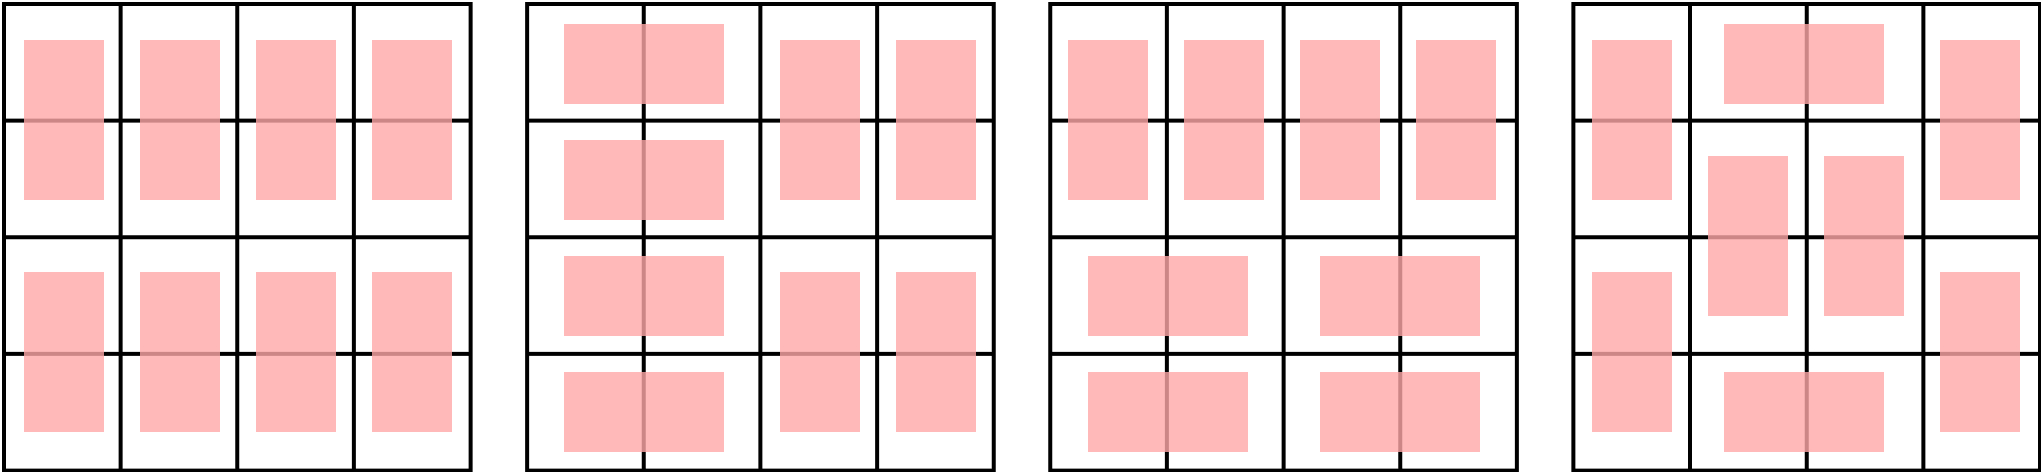
\includegraphics[scale=0.6]{Images/Figure1.jpg}
    \caption{$4$ out of the $36$ possible domino-tilings of a $4\times 4$ board.}
\end{figure}

Next, we state an equivalent formulation of \cref{q:1.7}.

\begin{definition}[Graph]
A graph is a pair $G=\left( V,E \right)$ where $V$ is a set whose elements are called vertices and $E$ is a set of unordered pairs of vertices whose elements are called edges.
\label{d:1.2}
\end{definition}

\begin{definition}[Perfect Matching]
Let $G=\left( V,E \right)$ be a graph. An $M\subseteq E$ is called a perfect matching of $G$ if no two edeges in $M$ share a common vertex and every vertex of $G$ is incident to atleast one edge in $M$.
\end{definition}
\begin{figure}[H]
	\centering
	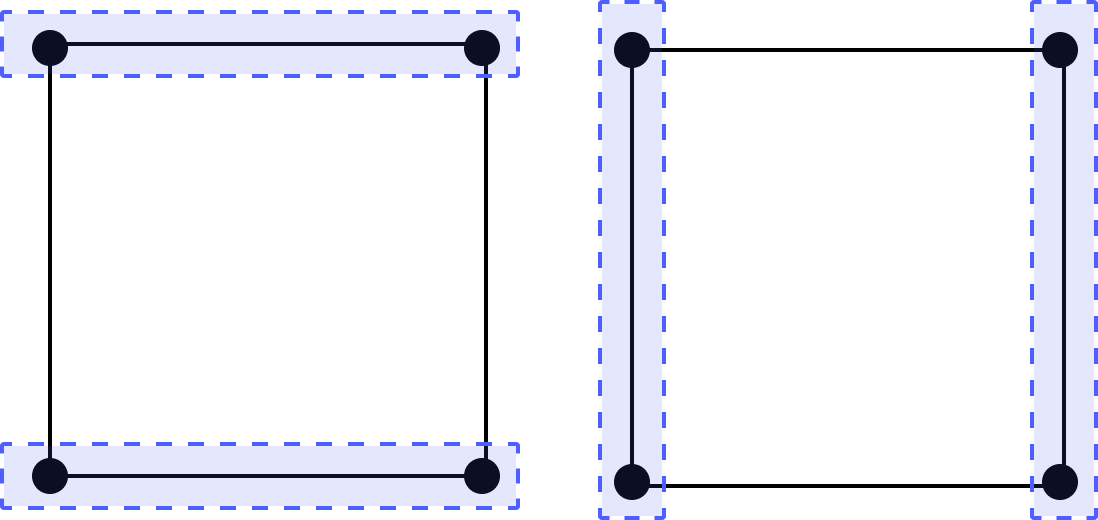
\includegraphics[scale=0.6]{Images/Figure2.jpg}
	\caption{The only possible perfect matchings of the grid graph of order $2$}
\end{figure}
Now consider the following construction. To each square in a given a board of order $m\times n$, we assign a vertex. Additionally, there is an edge between the said vertices if and only if the corresponding squares are adjacent to one another. \cref{f:1.3} is an example of this construction. 
\begin{figure}[H]
	\centering
	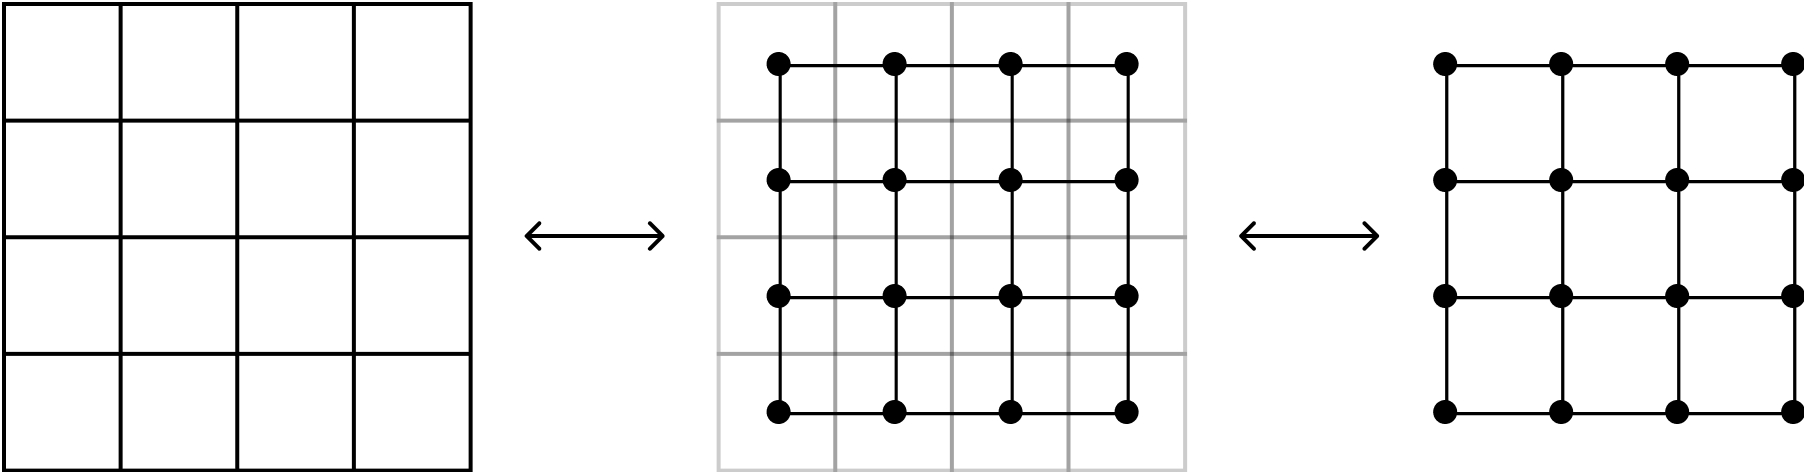
\includegraphics[scale=0.6]{Images/Figure3.jpg}
	\caption{A board of order $4\times 4$ and it's corresponding graph}
	\label{f:1.3}
\end{figure}
It is clear that our construction gives a one-to-one correspondence between the set of possible domino-tilings of a board and the set of perfect matchings of it's corresponding graph.
\begin{figure}[H]
	\centering
	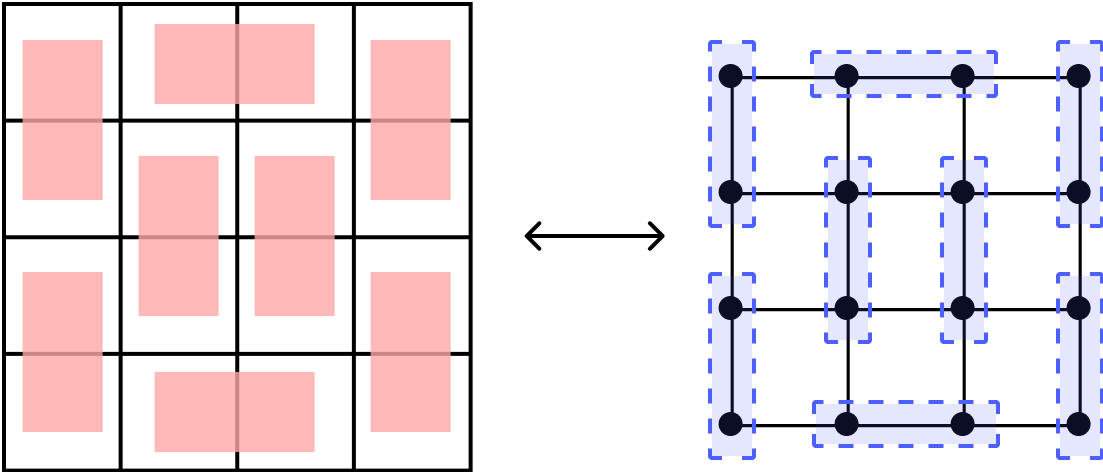
\includegraphics[scale=0.6]{Images/Figure4.png}
	\caption{A domino tiling of a board of order $4\times 4$ and the perfect matching that it admits}
\end{figure}
We shall revisit this formulation of the problem much later in the course. For now, restrict ourselves to a boards of order $2\times n$ and count the number of possible domino tilings, say $t_{n}$ as $n$ varies over the set of natural numbers. It is not too difficult to convince yourself of the fact that $t_{0}=1$, $t_{1}=1$, $t_{2}=2, t_{3}=3$, and $t_{4}=5$. Since the first five terms in the sequence $t_{n}$ are the same as the five terms of the Fibonacci sequence (say $F_{n}$), one might guess that $t_{n} = F_{n}$. This is indeed true, and we shall now give a proof of our claim using a counting argument.
\begin{figure}[H]
	\centering
	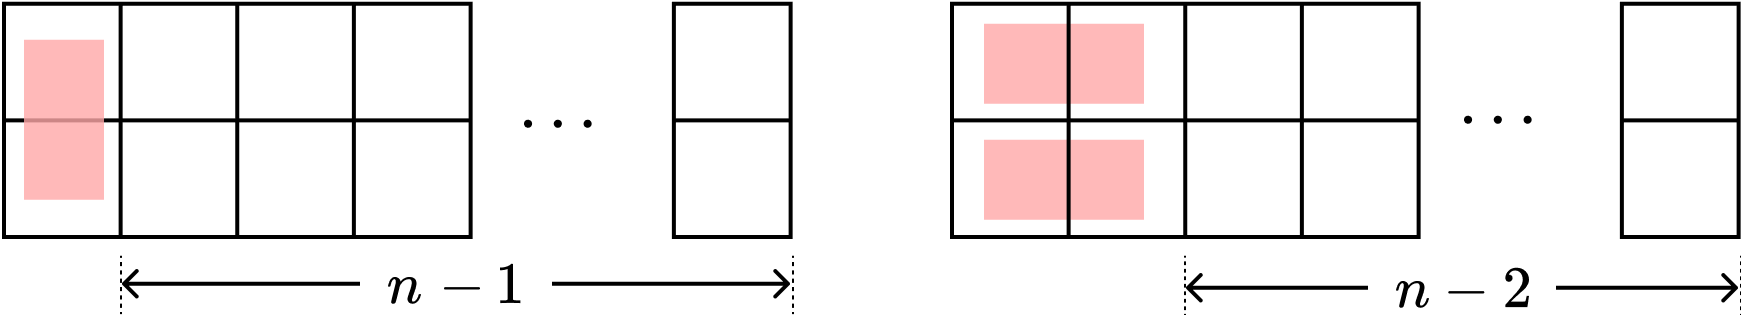
\includegraphics[scale=0.6]{Images/Figure5.png}
	\caption{Two ways to tile the first column of board of order $2\times n$}
	\label{f:1.4}
\end{figure}
\begin{proof}
	Notice how there are exactly two ways to tile the first column of any board of order $2\times n$ (refer to \cref{f:1.4}). It can either be tiled using a single vertical domino, in which case it remains to tile the sub-board of order $2\times \left( n-1 \right)$, or using two horizontal dominos, in which case it remains to tile the sub-board of order $2\times \left( n-2 \right)$. Since both of these cases are valid, it follows that \[
t_{n}=t_{n-1}+t_{n-2}
.\] Which is the same as the Fibonacci reccurence.
\end{proof}

Now that we have $F_{n}=t_{n}$, we prove two standard Fibonacci identities using counting arguments similar to the ones used in the above proof.

\begin{claim}
$F_{m+n}=F_{m}F_{n} + F_{m-1}F_{n-1}$
\label{c:1.1}
\end{claim}

\begin{proof}
\begin{figure}[H]
	\centering
	\begin{subfigure}[b]{0.3\textwidth}
		\centering
		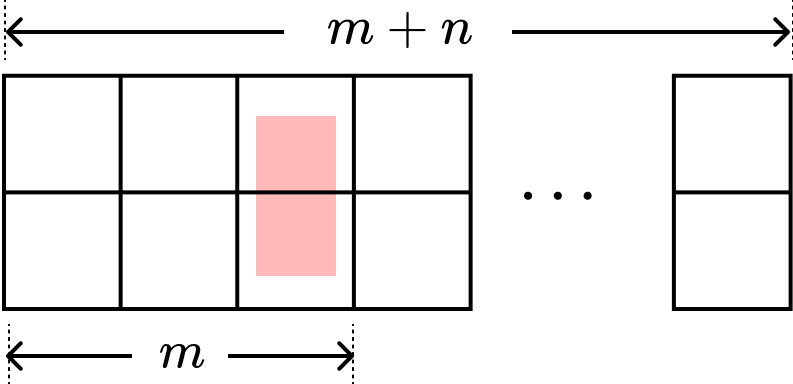
\includegraphics[scale=0.6]{Images/Figure6_1.png}
		\caption{}
	\end{subfigure}
	\hfill
	\begin{subfigure}[b]{0.3\textwidth}
		\centering
		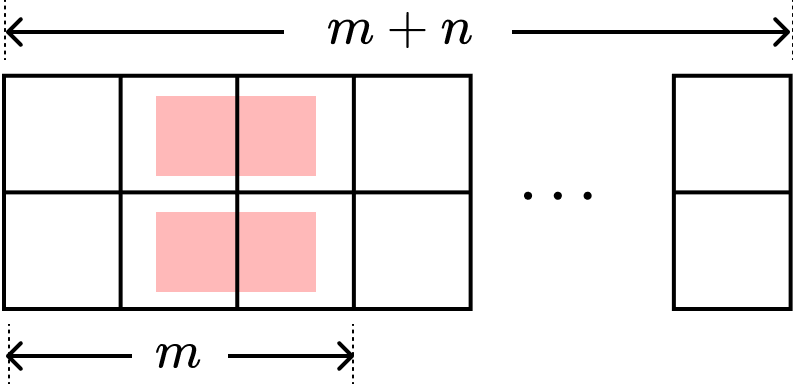
\includegraphics[scale=0.6]{Images/Figure6_2.png}
		\caption{}
	\end{subfigure}
	\hfill
	\begin{subfigure}[b]{0.3\textwidth}
		\centering
		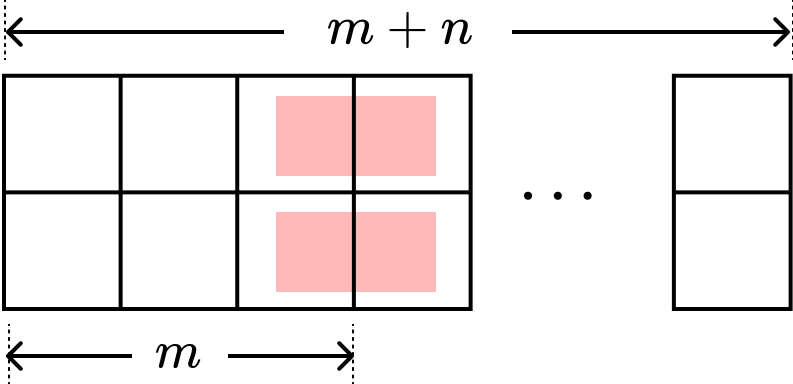
\includegraphics[scale=0.6]{Images/Figure6_3.png}
		\caption{}
	\end{subfigure}
	\caption{The only $3$ ways to tile the $m$-th row of a $2\times \left( m+n \right)$ board.}
	\label{f:1.6}
\end{figure}

Notice how we have exactly $3$ ways to tile the $m$-th row of a $2\times \left( m+n \right)$ board (refer to \cref{f:1.6}). Cases (a) and (b) account for when we have $F_{m}$ ways to tile the sub-block of order $2\times m$ \textbf{and} $F_{n}$ ways to tile the sub-board which occurs immediately after. Case (c), on the other hand, accounts for when we have $F_{m-1}$ ways to tile the sub-board of order $2\times \left( m-1 \right)$ which occurs before the already tiled $m$-th row  \textbf{and} $F_{n-1}$ ways to tile the sub-board of order $2\times \left( n-1 \right)$ which occurs after the already tiled $m$-th row. This proves the required identity.
\end{proof}

\begin{claim}
	$F_{0}+\cdots+F_{n} = F_{n+2}-1$
\end{claim}

\begin{proof}	
Notice how every board of order $2\times k$ has a trivial tiling; the one which only uses vertical dominos and no horizontal ones. On a board of order $2\times \left( n+2 \right)$ if this trivial tiling is ignored, every other possible tiling must have the occurence of atleast one pair of horizontal dominos. If the last such pair occurs at the $n+1$-th column, the sub-board of order  $2\times n$ preceeding it can be tiled in $F_{n}$ ways. If the last such pair occurs at the $n$-th column, the sub-board of order $2\times \left( n-1 \right)$ can be tiled in $F_{n-1}$ ways, and so on. This gives us the required identity. 
\end{proof}
\begin{figure}[H]
		\centering
		\begin{subfigure}[b]{0.3\textwidth}
			\centering
			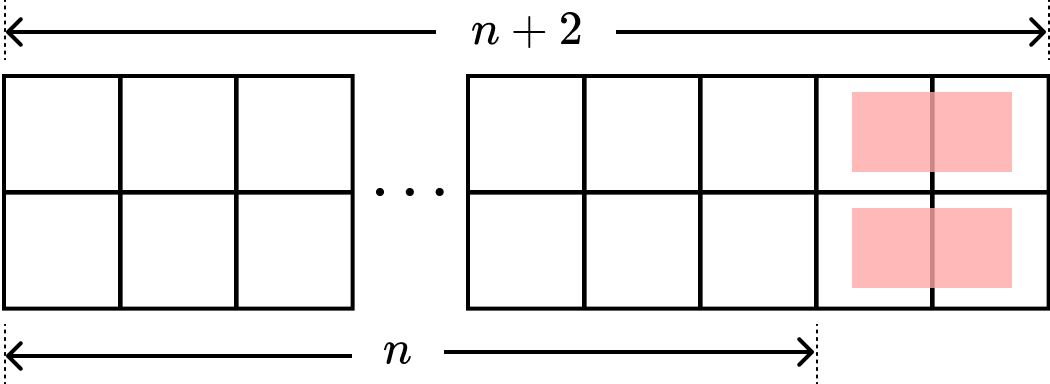
\includegraphics[scale=0.6]{Images/Figure7_1.png}
			\caption{}
		\end{subfigure}
		\vfill
		\begin{subfigure}[b]{0.3\textwidth}
			\centering
			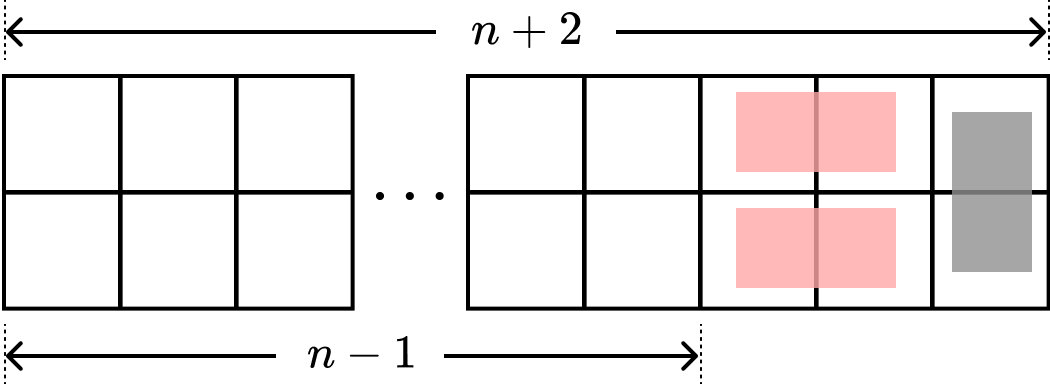
\includegraphics[scale=0.6]{Images/Figure7_2.png}
			\caption{}
		\end{subfigure}
		\vfill
		\begin{subfigure}[b]{0.3\textwidth}
			\centering
			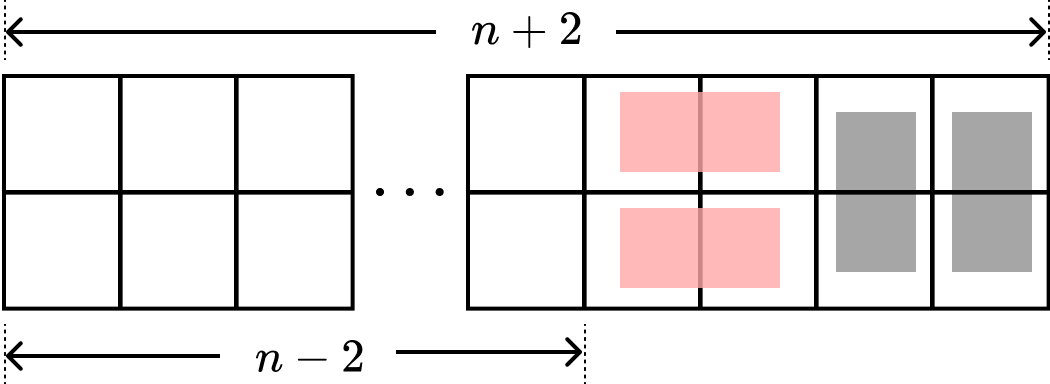
\includegraphics[scale=0.6]{Images/Figure7_3.png}
			\caption{}
		\end{subfigure}
\caption{Examples of occurences of the last pair of horizontal dominos in $3$ non-trivial tilings of a board of order $2\times \left( n+2 \right)$}
\label{f:1.7}
\end{figure}

Recall how $\binom{n}{k}$ counts the number of ways one can choose $k$ elements from a set of $n$ elements. We shall now state a rather interesting re-interpretation of binomial coefficients. 
\begin{figure}[H]
	\centering
	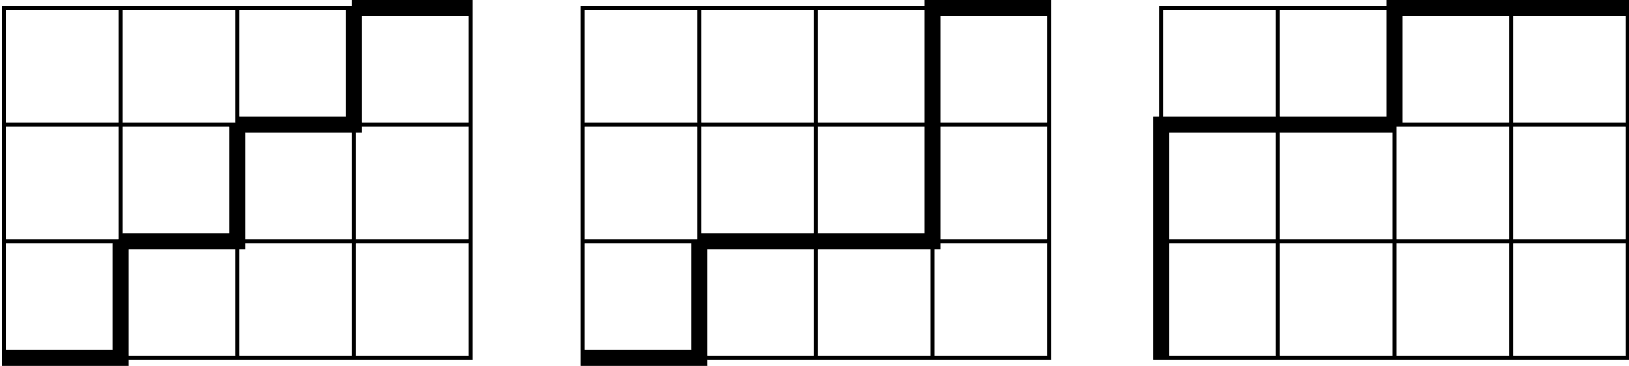
\includegraphics[scale=0.6]{Images/Figure8.png}
	\caption{$3$ examples of lattice paths from $\left( 0,0 \right)$ to $\left( 4,3 \right) $}
	\label{f:1.8}
\end{figure}
\begin{question}
Given that the only moves allowed are North (N), corresponding to $\left( i,j \right) \to \left( i,j+1 \right)$, or East (E), corresponding to $\left( i,j \right)\to \left( i+1,j \right)$, count the number of paths from $\left( 0,0 \right)$ to $\left( m,n \right)$ on a grid of order $m\times n$ (refer to \cref{f:1.8} for examples of such paths).
\label{q:1.8}
\end{question}
\begin{solution}
Notice how we require exactly $m$ E-moves and $n$ N-moves to reach $\left( m,n \right)$ from $\left( 0,0 \right)$. However, every lattice path is determined completely by a choice of $m$ E-moves (or equivalently $n$ N-moves) which can be made in $\binom{m+n}{m}$ ways (or equivalently $\binom{m+n}{n}$ ways).
\end{solution}
\begin{remark}
As a consequence of this counting exercise we have not only given a re-interpretation of binomial coefficients, but have also proved that they are symmetric, i.e, $\binom{n}{k}=\binom{n}{n-k}$.
\label{r:1.2}
\end{remark}
Per usual, we are now interested in giving a counting argument for a standard identity concerning binomial coefficients called Pascal's identity.
\begin{claim}
$\binom{n}{k} + \binom{n}{k+1} = \binom{n+1}{k+1}$
\label{c:1.3}
\end{claim}
\begin{proof}
Notice how there are $\binom{n+1}{k+1}$ choices of a lattice paths from $\left( 0,0 \right)$ to $\left( n-k,k+1 \right)$. The last step in each one of these paths is either an N-move or an E-move. If it is an N-move then it suffices to choose one lattice path from $\left( 0,0 \right)$ to $\left( n-k-1,k+1 \right)$ out of the \[
\binom{\left( n-k-1 \right) + \left( k+1 \right)}{k+1} = \binom{n}{k+1}
\] choices. Alternatively, if it is an E-move then it suffices to choose one lattice path from $\left( 0,0 \right)$ to $\left( n-k,k \right)$ out of the \[
\binom{\left( n-k \right) + k}{k} = \binom{n}{k}\] choices.
\end{proof}
Let's remind ourselves that the central objective of this course is to count. From \cref{q:1.1} through \cref{q:1.6}, we encountered examples where we derived exact closed-form expressions for counting. During our discussion of the dimer model, we first stated a closed-form expression and then constructed a bijection between the tiling configuration and the perfect matchings configuration. By restricting ourselves to boards of size $2 \times n$, we demonstrated that finding a recurrence relation is also a valid counting technique. However, as we will see, the methods we have discussed so far are not always applicable. In such cases, we turn to the idea of generating functions, which we will introduce next.

\begin{definition}[Ordinary Generating Function]
	Given a sequence $\{a_{n}\}_{n \ge 0}$ the formal power series, $\sum_{k=0}^{\infty}a_{k}x^k$, in an indeterminate $x$ is called the generating function of $\{a_{n}\}_{n \ge 0}$.
 \label{d:1.4}
\end{definition}

Since our definition works with a \textit{formal} power series we need not worry about the divergence of the involved infinite sum. That being said, we can always be cautious and assume $|x|<1$ to guarantee convergence. 

\begin{question}
	Find the generating function for the sequence of Fibonacci numbers. 
 \label{q:1.9}
\end{question}
\begin{solution}
Let $\{f_{n}\}_{n \ge 0}$ denote the sequence of Fibonacci numbers and let $F\left( x \right)$ be the corresponding generating function. Notice how 
\begin{align*}
	F\left( x \right) &= \sum_{k=0}^{\infty} f_{k}x^k \\
	&= f_{0}+f_{1}x+\sum_{k=2}^{\infty}f_{k}x^k \\
	&= 1+x+\sum_{k=2}^{\infty}f_{k}x^k \\
	&= 1+x+\sum_{k=2}^\infty \left( f_{k-1}+f_{k-2} \right) x^k \\
	&= 1+x+\sum_{k=2}^{\infty} f_{k-1}x^k + \sum_{k=2}^{\infty} f_{k-2}x^k \\
	&= 1+x+x\left( F\left( x \right) -1 \right) + x^2F\left( x \right)  \\
	&= 1+xF\left( x \right)+x^2F\left( x \right)
\end{align*}
Solving which we obtain \[
F\left( x \right) = \frac{1}{1-x-x^2}
\].
\end{solution}
Throughout this course, we will explore how and why generating functions are extensively used in combinatorics. We introduce one such instance now, which will be discussed in greater depth later.
\begin{definition}
An integer partition of a natural number $n$ is a non-increasing sequence of natural numbers, $\{\lambda_i\}_{i \ge 1}$, whose sum is $n$.
\label{d:1.5}
\end{definition}
\begin{question}
In how many ways can a natural number $n$ be partitioned?
\end{question}
Let $p(n)$ denote the number of partitions of $n$. Interestingly, no "nice" closed-form expression for $p(n)$ has been found. However, we will derive the generating function \[
	\prod_{n=1}^\infty\left( 1+x^n +x^{2n}+x^{3n}+\cdots\right) =  \sum_{n=0}^{\infty}p\left( n \right) x^n
\] which was given by Euler, later in the course.
\begin{remark}
In the year 1918, G.H Hardy and Srinivasa Ramanujan obtained an asymptotic expression (an expression which describes the limiting behaviour) for $p\left( n \right)$ which is given by \[
p\left( n \right) ~ \frac{1}{4n\sqrt{3}}\exp\left( \pi \sqrt{\frac{2n}{3}}  \right) .\] Oftentimes stating an asymptotic expression is also a valid counting technique.
\label{r:1.3}
\end{remark}
\section{Counting Principles}
We state the fundamental counting principles now.
\begin{enumerate}
\item (Addition Principle): If $\{A_{k}\}_{k\geq 1}$ is a family of finite and pairwise disjoint sets then $\abs{\bigcup_{k\geq 1} A_{k}} = \sum_{k\geq 1}\abs{A_{k}}$.
\item (Substraction Principle): If $A$ and $B$ are finite sets such that $B\subseteq A$ then $\abs{A\backslash B} = \abs{A}-\abs{B}$.
\item (Product Rule): If $A$ and $B$ are finite sets, then $\abs{A\times B} = \abs{A}\cdot\abs{B}$.
\item (Division Rule): For finite sets $A$ and $B$ if there exists a $d$-to-many function $f:A\to B$ then $\abs{B}=\abs{A}/d$.
\end{enumerate}
In some sense we've already been using these principles in disguise thus far. For instance;
\begin{question}
How many $k$-digit positive numbers are there?
\end{question}
\begin{solution}
Since we have $10$ choices for the first $\left(k-1\right)$ digits and $9$ choices for the last digit, by the product rule there are $9\cdot 10^{k-1}$ $k$ digit numbers.
\end{solution}
This is a good point to recall the binomial theorem and prove it using a counting argument instead of the standard induction argument.
\begin{theorem}[Binomial Theorem]
	\[
		\left( x+y \right)^n = \sum_{k=0}^{n}\binom{n}{k}x^{n-k}y^k
	.\] 
\end{theorem}
\begin{proof}
	Consider the expansion of
	\[
		\left( x+y \right)^n = \underbrace{\left( x+y \right) \cdots \left( x+y \right) }_{n \text{ factors}}.
	\]
	In this expansion, there are $\binom{n}{k}$ ways to choose $x$ from exactly $k$ of the $n$ factors (which forces the choice of $y$ from the remaining $(n-k)$ factors). Since $k$ can range from $0$ to $n$, applying the addition principle gives us the binomial theorem.
\end{proof}
Now we state the multinomial theorem which generalizes the binomial theorem to expressions with more than two terms, allowing us to expand any power of a sum of multiple terms as a sum of products of those terms, each multiplied by a what is called a multinomial coefficient which is denoted and defined as
\[\binom{n}{k_1,\cdots,k_m} := \frac{n}{k_1!\cdots k_m!}.\]
Next, we state an identity concerning multinomial coefficients which would help us prove the multinomial theorem. 
\begin{claim}
\[
\binom{n}{k_{1},\cdots,k_{r}} = \binom{n}{k_{1}}\binom{n-k_{1}}{k_{2}} \cdots \binom{n-k_{1}-\cdots-k_{r-1}}{k_{r}}
\]
\label{c:2.1rev}
\end{claim}
\begin{proof}
The proof follows simply by expanding the R.H.S out.
\begin{align*}
\binom{n}{k_{1}}\cdots \binom{n-k_{1}-\cdots-k_{r-1}}{k_{r}} &= \dfrac{n!}{(n-k_1)!k_1!}\dfrac{(n-k_1)!}{(n-k_1-k_2)!k_2!} \cdots \dfrac{(n-k_1-\cdots-k_{r-1})!}{(n-k_1-\cdots-k_{r})!k_r!} \\
&= \dfrac{n!}{k_1!\cdots k_r!}\dfrac{(n-k_1)!\cdots (n-k_1-\cdots-k_{r-1})!}{(n-k_1)!\cdots (n-k_1-\cdots-k_{r-1})!} \\
&=\dfrac{n!}{k_1!\cdots k_r!} \\
&=\binom{n}{k_1,\cdots,k_r}
\end{align*}
\end{proof}
We would expect the multinomial coefficient to count something. That is indeed the case, it counts the number of ways to arrange $n$ distinct objects into $m$ distinct bins such that the $i$-th bin contains $k_i$ elements. With this interepretation of multinomial coefficients, and \cref{c:2.1rev}, mimicing the steps involved in the proof of the binomial theorem we get the multinomial theorem which is stated below. 
\begin{theorem}[Multinomial Theorem]
	\[
	(x_{1}+\cdots+x_{r})^n = \sum_{k_{1}+\cdots+k_{r}=n}\binom{n}{k_{1},\cdots,k_{r}}x_{1}^{k_{1}}\cdots x_{r}^{k_{r}}
	.\] 
\end{theorem}
It is natural to expect a Pascal-like identity for multinomial coefficients as well. In this spirit, we state the following claim.
\begin{claim}
	\[
		\binom{n}{k_{1},\cdots,k_{r}} = \binom{n-1}{k_1-1,k_2,\cdots,k_r} + \cdots + \binom{n-1}{k_1,k_2,\cdots,k_r-1}
	.\]
\end{claim}
\begin{remark}
Notice how when $k_1=k$, $k_2=n-k$ and all the other $k_i$s are $0$, we retrieve the Pascal's identity (\cref{c:1.3})    
\end{remark}
This is a good point to introduce ourselves to yet another generalization of the binomial theorem which deals with the expansion of $(x+y)^n$ where $n$ is allowed to take complex values. 
\begin{theorem}[Generalized Binomial Theorem]
For all $n\in\mathbb{C}$ we have
\[
(1+x)^n = \sum_{k\geq 0}\binom{n}{k}x^k
\]
\label{t:2.3rev}
\end{theorem}
\begin{remark}
There are two well-known proofs of \cref{t:2.3rev}. One uses the idea of Taylor's series expansion, and the other uses the solution to a differential equation called the Legendre's equation. We state neither one of them here.  
\end{remark}
In addition to the fundamental counting principles, there are a few more principles/techniques which we will use quite often in this course. One of them is the bijection principle. We state the principle formally and then given an example.
\begin{theorem}[Bijection Principle]
If $S$ and $T$ are finite sets then $|S|=|T|$ if and only if there exists a bijection $f:S\to T$.
\end{theorem}
\begin{question}
Let $S$ be a finite set. A \textbf{permutation} of $S$ is a bijection from and to $S$. How many permutations of $[n]=\{1,2,3,\ldots,n\}$ exist?
\end{question}
We introduce the cycle notation before outlining a solution. In the case where $n=1$, it is clear that there is only possible bijection, namely, $f_1:\{1\}\to\{1\}$ such that $f_1 \left(1 \right) =1$. We shall write $f_1$ as \[
\begin{pmatrix}
	1 \\ 1
\end{pmatrix}
.\] In the case where $n=2$, it is clear that there are two possible bijections. These are $g_1:\{1,2\}\to \{1,2\}$ such that $g_1\left(1 \right) =1$, $g_1\left( 2 \right)=2$, and $g_{2}:\{1,2\}\to\{1,2\}$ such that $g_{2}\left(1  \right) =2$, $g_{2}\left( 2 \right) =1$. We shall write $g_{1}$ and $g_{2}$ as \[
\begin{pmatrix} 1 & 2 \\ 1 & 2 \end{pmatrix}, \quad \begin{pmatrix} 1 & 2 \\ 2 & 1 \end{pmatrix} 
\] respectively. In essence, the first row in our notation lists the elements of the domain, and the second row lists where the bijection sends these elements. Do you see why in the case where $n=3$ the bijections can be written as 
 \[
	 \begin{pmatrix} 1 & 2 & 3 \\ 1 & 2 & 3 \end{pmatrix}, \begin{pmatrix} 1 & 2 & 3 \\ 1 & 3 & 2 \end{pmatrix}, \begin{pmatrix} 1 & 2 & 3 \\ 2 & 1 & 3 \end{pmatrix}, \begin{pmatrix} 1 & 2 & 3 \\ 2 & 1 & 3 \end{pmatrix}, \begin{pmatrix} 1 & 2 & 3 \\ 2 & 3 & 1 \end{pmatrix}, \begin{pmatrix} 1 & 2 & 3 \\ 3 & 1 & 2\end{pmatrix}, \begin{pmatrix} 1 & 2 & 3 \\ 3 & 2 & 1 \end{pmatrix} 
.\]
Since the first row of any bijection in our notation is fixed and we have \[ n\cdot\left( n-1 \right) \cdots 1 = n!\] ways to fill out the second row, it clear that there are $n!$ permutations of $[n]$. Recall from \cref{q:1.5} that we also have exactly $n!$ permutation matrices. By the bijection principle we must have a bijection between the set of permutation matrices of order $n\times n$ and the set of permuations of $[n]$. The bijection is as follows. Corresponding to every permutation \[
\begin{pmatrix} 
	1 & 2 & \cdots & n \\
	f\left(1\right) & f\left( 2 \right) & \cdots & f\left( n \right)
\end{pmatrix} 
\] of $[n]$ we assign an $n\times n$ matrix where the entry at $\left( i,f\left(i  \right)  \right)$ for $1\leq i\leq n$ is $1$, and all other entries are $0$. More explicity,
\begin{align*}
    &\begin{pmatrix}
    1 & 2 & 3 \\
    1 & 2 & 3 
\end{pmatrix}
\longleftrightarrow
\begin{pmatrix}
    1&& \\
    &1& \\
    &&1
\end{pmatrix}, \\
&\begin{pmatrix}
    1 & 2 & 3 \\
    1 & 3 & 2 
\end{pmatrix}
\longleftrightarrow
\begin{pmatrix}
    1&& \\
    &&1 \\
    &1&
\end{pmatrix}, \\
&\hspace*{6em}\vdots \\
&\begin{pmatrix}
    1 & 2 & 3 \\
    3 & 2 & 1
\end{pmatrix}
\longleftrightarrow
\begin{pmatrix}
    &&1\\
    &1&\\
    1&&
\end{pmatrix}.
\end{align*}
We outline a proof of an identity involving binomial coefficients using the bijection principle now.
\begin{claim}
\begin{align*}
\sum_{i=0}^{n}\binom{n}{i} = 2^n
\end{align*}
\label{c:2.1}
\end{claim}
\begin{proof}
	Let \( S = \{a_1, \ldots, a_n\} \) be a set with \( n \) elements. For each of the \( 2^n \) possible subsets \( T = \{a'_1, \ldots, a'_k\} \) of \( S \) (where \( k \) can be any value from 0 to \( n \)), there is a corresponding binary string of length \( n \). In this string, the \( i \)th bit is \( 1 \) if the element \( a_i \) is in the subset \( T \), and \( 0 \) if it is not. For instance in the case where $S=\{0,1\}$ we have the following correspondence
	 \begin{align*}
		&\emptyset \longleftrightarrow 00 \\
		&\{0\} \longleftrightarrow 10 \\
		&\{1\} \longleftrightarrow 01 \\
		&\{0,1\} \longleftrightarrow 11
	\end{align*}
\end{proof}
Another counting technique which we've seen before in the proof of Pascal's identity (\cref{c:1.3}) is called double counting. The broad idea is to count the same combinatorial object in two different ways. As an example, we give a proof of \cref{c:2.1} using the double counting technique.
\begin{proof}
It is clear that $2^n$ counts the number of $n$-bit binary strings. To prove the claimed identity, we count the number of $n$-bit binary strings once again in a different way. Notice how an arbitrary$n$-bit binary string has $0\leq i\leq n$ number of $0$s. Since there are $\binom{n}{0}$ choices when $i=0$, $\binom{n}{1}$ choices when $i=1$, and so on, by the addition principle we have proved the required identity.
\end{proof}
We have all seen a proof by induction of the following identity. Now we give a proof using a double counting argument.
\begin{claim}
	$1+2+3+\cdots+n=\dfrac{n\left( n+1 \right)}{2}=\binom{n+1}{2}$
	\label{c:2.2}
\end{claim}
\begin{proof}
Consider the problem of counting the number of handshakes in a group of $n+1$ people, where each person shakes hands with every other person. The first person in the group shakes hands with everyone except themselves; this gives $n$ handshakes. The second person in the group shakes hands with everyone else; this gives $\left( n-1 \right)$ handshakes (not $n$ because we've already counted the handshake between the first and second person). The third person in the group shakes hands with everyone; this gives $\left( n-2 \right)$, and so on. In all we have $n+\left( n-1 \right)+\left( n-2 \right)+\cdots+1$ handshakes. Let's count again in a different way now. Notice how for each pair of people there is one handshake. Hence, there are $\binom{n+1}{2}$ handshakes in total. Putting the two observations together proves the claim.
\end{proof}
Next, we introduce the ``Stars-and-Bars'' method. We shall outline how this method works with the help of a standard example.
\begin{question}
For a given $n\in \mathbb{N}$ find the number of solutions to the equation  $x_{1}+\cdots+x_{k}=n$ where $n\in\mathbb{N}$ and  $x_{i}\in\mathbb{Z}$?
\label{q:2.3}
\end{question}
\begin{solution}
Recall how in the definition of partition (\cref{d:1.5}), the order of the parts did not matter, i.e, the partitions $2+1$ an $1+2$ of $3$ are the same to us. Partitions where the order does matter are called compositions. Compositions where $0$s are allowed to be a part are called weak compositions. With these two definitions at hand, notice how there are two cases to deal with in $\cref{q:2.3}$.
\begin{enumerate}
    \item All $x_{i}>0$; which is equivalent to counting the number of compositions of $n$ into $k$ parts.
    \item All $x_{i}\geq 0$; which is equivalent to counting the number of weak compositions of $n$ into $k$ parts.
\end{enumerate}
Let $x_1+\cdots+x_k=n$ be a composition (may or may not be weak) of $n$ into $k$ parts. Now we replace each $x_i$ with $x_i$ consecutive stars, and each $+$ with a bar. For instance, the composition $5+3+1$ would be written as \[
***** \ | \ *** \ | \ *
\] and the (weak) composition $5+3+1+0$ would be written as 
\[
***** \ | \ *** \ | \ * \ | \ |.
\]
Since every composition (may or may not be weak) of $n$ into $k$ parts is completely determined by an arrangement of $n$ stars and $k-1$ bars, it is clear that we have $\binom{n+k-1}{k-1}$ weak compositions and $\binom{n-1}{k-1}$ compositions.
\end{solution}
\begin{remark}
Notice how every weak composition $n=d_1+\cdots+d_k$ of $n$ into $k$ parts naturally corresponds to the monomial degree $n$ in $k$ variables given by $x_1^{d_1}\cdots x_k^{d_k}$.
\end{remark}
We conclude this section by stating an informal technique called proof by pictures (or proof without words). This technique involves the use of visual representations to demonstrate the validity of a mathematical statement. Although in the strictest sense of things a proof by pictures is not a counting principle, it often helps develop intution. For instance, we state such a proof for \cref{c:2.2}. 
\begin{proof} 
	\begin{figure}[H]	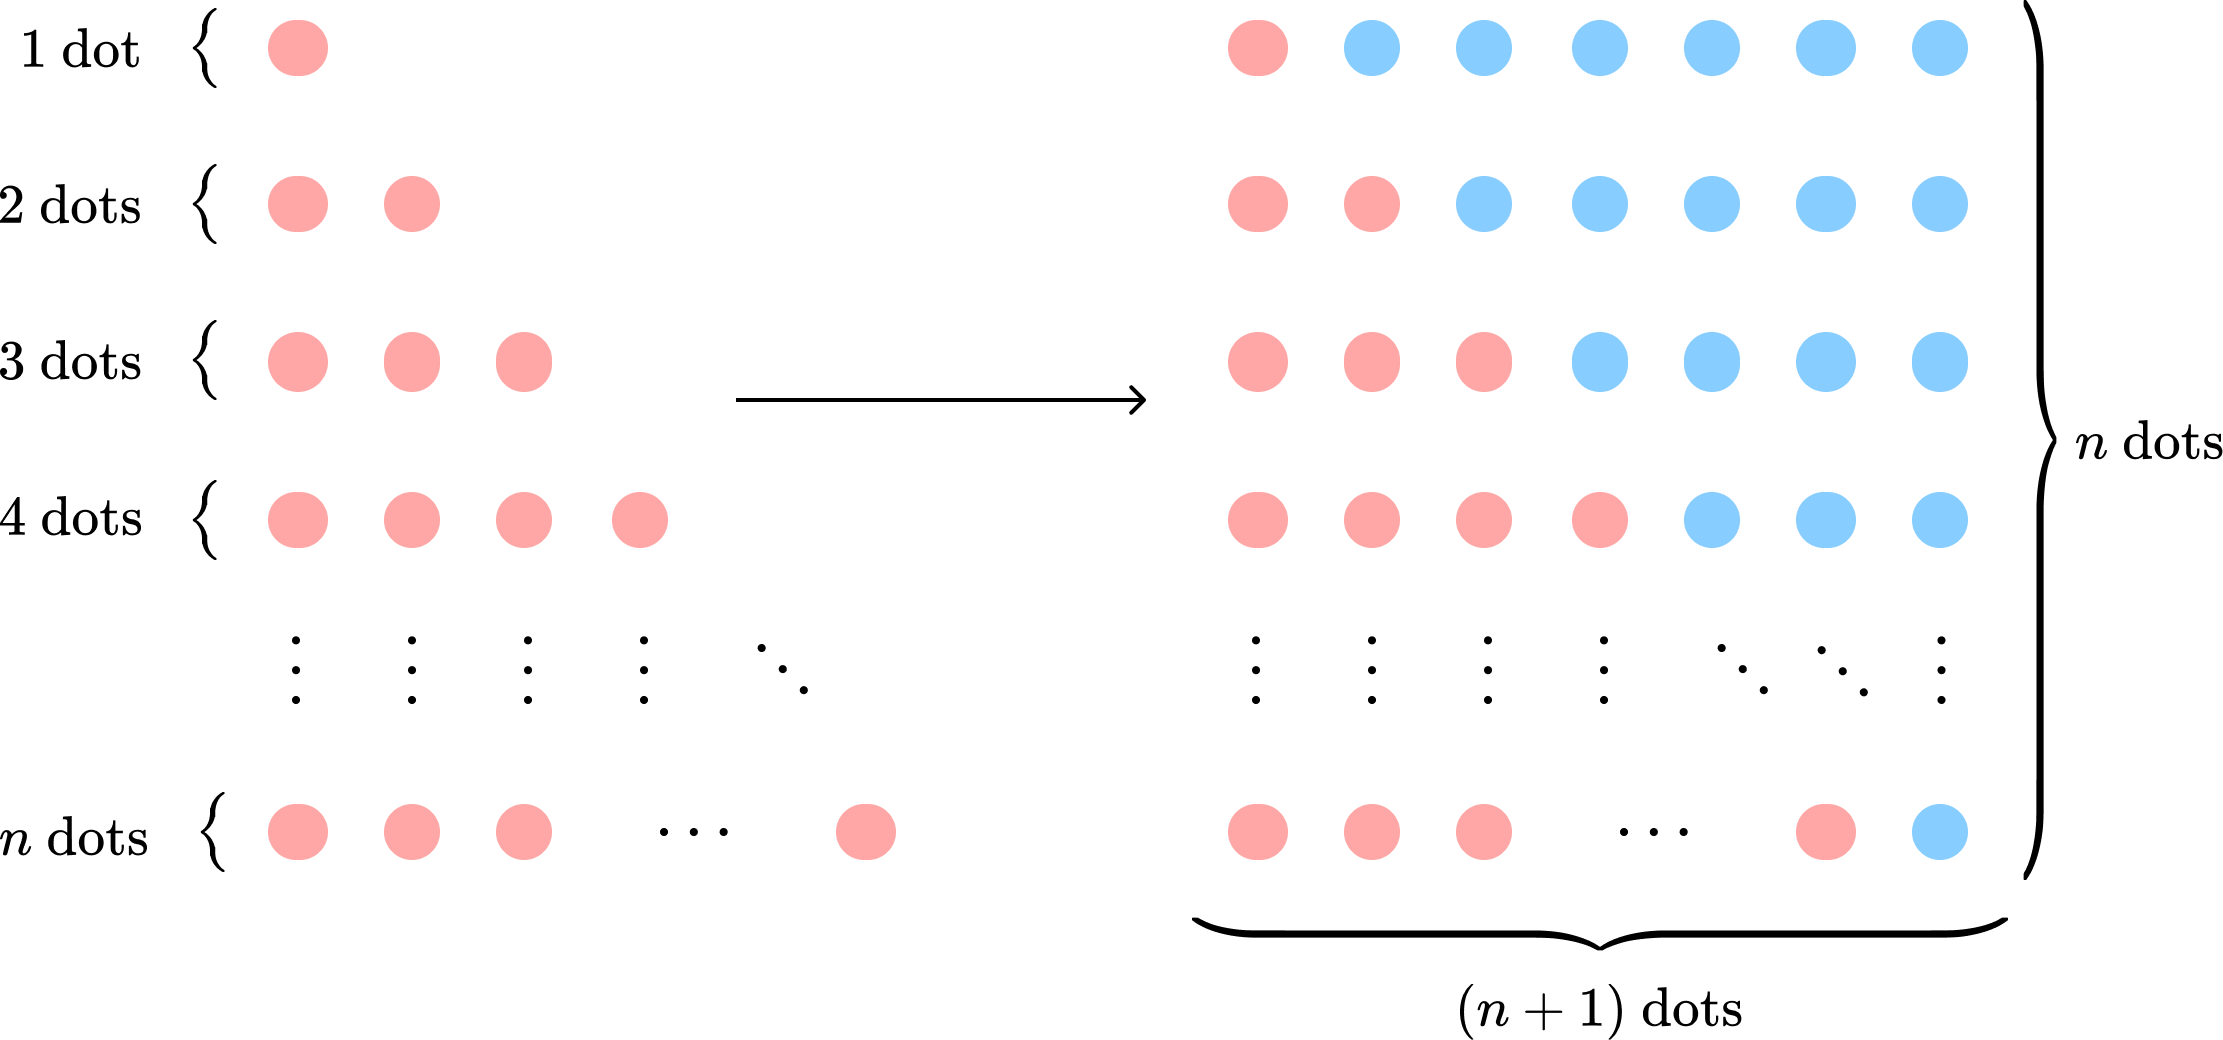
\includegraphics[scale=0.65]{Images/Figure9.png}
		\caption{}
		\label{f:1.9}
	\end{figure}
In \cref{f:1.9} notice how there are $1+2+3+\cdots+n$ dots colored in red, $1+2+3+\cdots+n$ dots colored in blue, and hence $2\left( 1+2+3+\cdots+n \right)$ total. It is also true that in our arrangement there are $n\left( n+1 \right)$ dots in total. Now the identity follows.
\end{proof}
Yet another fundamental counting principle is the pigeon-hole principle. Given its importance, we will dedicate the upcoming section to explore it in detail.
\begin{remark}
We have seen how the principles we’ve discussed so far can be useful in proving combinatorial identities. Determining how to derive these identities is not always straightforward. However, a common technique involves running computer simulations to generate a sequence of values corresponding to the first few natural numbers. Tools like OEIS, RATE (in Mathematica), and Guess (in SageMath and Maple) can then be used to conjecture a closed form for the sequence.
\end{remark}

\begin{comment}
-------
Challenge problems:
-----
$t_{n} = \binom{n}{0}+\binom{n-1}{1}+\binom{n-2}{2} + \cdots$
$\binom{2n}{n} = \sum_{k=0}^{n}\binom{n}{k}^2$

Consdier a $4 x 4$ chessboard. We want to place as many queens as possible such that they don't attack each other. What are the possible number of such configurations. What are the maximum number of queens you can place? Show that it has to be less than $5$. Give two examples of configurations with $4$ queens. This works only for chessboard greater than $4$ (i.e order n and n queens).
\end{comment}

\section{The Pigeon-hole Principle}
We state what is known as the pigeon-hole principle.
\begin{theorem}[Pigeon-hole Principle]
Let $A_{1},\cdots,A_{k}$ be pair-wise disjoint finite sets. If \[|A_{1}\cup A_{2}\cup \cdots \cup A_{k}|>kr\] then there exists an $1\leq i\leq k$ such that $|A_{i}|>r$.
\end{theorem}
Even though the statement sounds trivial, it has immense applications. We state a few examples now. 
\begin{claim}
Given $b\in \mathbb{Z}$, the decimal expansion of $1/b$ is either finite or eventually periodic.
\end{claim}
\begin{proof}
Each step in the long division of $1$ by $b$ involves subtracting multiples of $b$ from powers of $10$ until the remainder is $0$ or repeats itself. Since each one of these remainders must be strictly less than $b$, we have $b$ possible remainders, namely, $0, 1, 2, \cdots, b-1$. If the remainder becomes $0$ at some step, the division terminates, in which case the decimal expansion is finite. Next, consider the case where the division does not terminate. By the pigeon-hole principle, since there are only $b$ possible remainders and more than $b$ steps, at least one of the remainders must repeat. This proves our claim because when a remainder repeats, the sequence of digits that follow in the decimal expansion must repeat as well.
\end{proof}
\begin{claim}
Let $S=\{1,2,\cdots,2n\}$. Any $n+1$ element subset $K$ of $S$ has two co-prime numbers, and two numbers such that one is an integer multiple of the other. 
\end{claim}
\begin{proof}
Consider the $n$-element subset $\{\left( 1,2 \right), \left( 3,4 \right), \cdots \left( 2n-1,2 \right)\}$ of $S\times S$ and notice how if we choose $n+1$ numbers from $\{0,\cdots,2n\}$ then by the pigeon-hole principle we are guaranteed to pick two numbers from the same pair in $S\times S$. Since each element in the said subset is a pair of consecutive numbers, their $\gcd$ is necessarily $1$. Next, notice how every element in the set $\{1,2,\cdots,2n\}$ can be written in the form $2^ab$ where $b$ is odd by factoring out as many $2$s as possible. Since there are only $n$ odd numbers in these set $\{1,2,\cdots,2n\}$, we are left with $n$ choices of $b$. Next, we construct $b$ subsets of $S$, say $S_k\subseteq S$ such that $i\in S_k$ if and only if $i=2^kb$. Finally, by the pigeon-hole principle, if one were to pick $n+1$ elements from $S$ atleast $2$ of them would be in the same $S_k$, i.e, there always exists a pair of numbers such that one divides the other.
\end{proof}
\begin{claim}
If $S$ be an $n+1$-element set of natural numbers, then there exists a pair of numbers in $S$ whose difference is divisible by $n$.
\end{claim}
\begin{proof}
Notice how the remainder obtained upon dividing any element $a_i\in S=\{a_1,\cdots,a_{n+1}\}$ by $n$ must be one of $0,1,\cdots,n-1$. Since there are $n+1$ $a_i$s but only $n$ possible remainders, by the pigeon-hole principle, atleast two members (say $a_i$ and $a_j$)in $S$ must have the same remainder, i.e, $a_i = nq_1 + r$ and $a_j = nq_2 + r$ for some natural numbers $q_1$ and $q_2$ and $0\leq r\leq n-1$. Clearly, $a_i-a_j = n(q_1-q_2)$ is divisible by $n$.
\end{proof}
\begin{claim}
Given $m$ integers say $a_{1},\cdots,a_{m}$ there exists $k$ and $l$ with  $0\leq k\leq l\leq m$ such that $m$ divides $a_{k+1}+a_{k+2}+\cdots+a_{l}$
\end{claim}
\begin{proof}
Consider sums of the form $\sum_{i=1}^{k}a_i$ for $1\leq k\leq m$. If one of these sums is divisible by $m$, i.e, their remainder upon division by $m$ is $0$ then we are done. If not, we have $m-1$ possible remainders for the said sums, namely, $1,2,\cdots m-1$. Since there are $m$ possible sums and only $m-1$ possible remainders atleast two of these sums share the same remainder. More specifically, for some $1\leq r<s\leq m$ and integers $q_1,q_2$ we have $\sum_{i=1}^{r}a_i = nq_1 + r$ and $\sum_{i=1}^{s}a_i = nq_2 + r$. But then clearly, $\sum_{i=r+1}^{s}a_j = n(q_1-q_2)$ is divisible by $n$ and we are done.
\end{proof}
\begin{question}
In a party of $n$ people, where some (maybe all, maybe none) shake hands with one another, show that there are atleast two people who shake the same number of hands.
\end{question}
\begin{solution}
Consider the case where each one of the $n$ people shake hands at least once. The number of handshakes possible for everybody then is $n-1$. Since there are $n$ people in the party, by the pigeon-hole principle our claim holds true. If we don't assume that everyone shakes at least one hand then we can separate the $n$ people between $k$ people who don't shake any hands and $m$ people who do, and the problem is reduced to the last case with $n=m$.
\end{solution}
\begin{question}
In a group of $6$ people where each pair of people are either friends or enemies, show that there are $3$ people who are either all friends or all enemies. 
\label{q:3.2}
\end{question}
\begin{solution}
Let $A,B,C,D,E$ and $F$ be a group of $6$ friends. Pick $A$, and notice how each one of the remaining $5$ people is either a friend of $A$ or an enemy of $A$. Now, by the pigeon-hole at least three of them (say $B,C$ and $D$) are either friends of $A$, or enemies of $A$. We consider the case where they are friends of $A$ and the other case will follow similarly. If any one of the pairs $B$-and-$C$, $C$-and-$D$, or, $B$-and-$D$ are friends, then we have found a group of $3$ people who are all friends. If neither one of the pairs $B$-and-$C$, $C$-and-$D$, or, $B$-and-$D$ are friends, then we have found a group of $3$ people who are all enemies.
\end{solution}
We state an interesting graph-theoretic (recall \cref{d:1.2}) restatement of \cref{q:3.2} now. Let the group of $6$ be represented as vertices in a graph. For each pair of these vertices, let there be an edge connecting them, which is colored red if the two represented people are enemies and blue if they are friends. Now \cref{q:3.2} asserts that now matter how you color the (edges of the) graph, there is always a ``triangle'' of the same color in the graph. 
\begin{figure}[H]
    \centering
    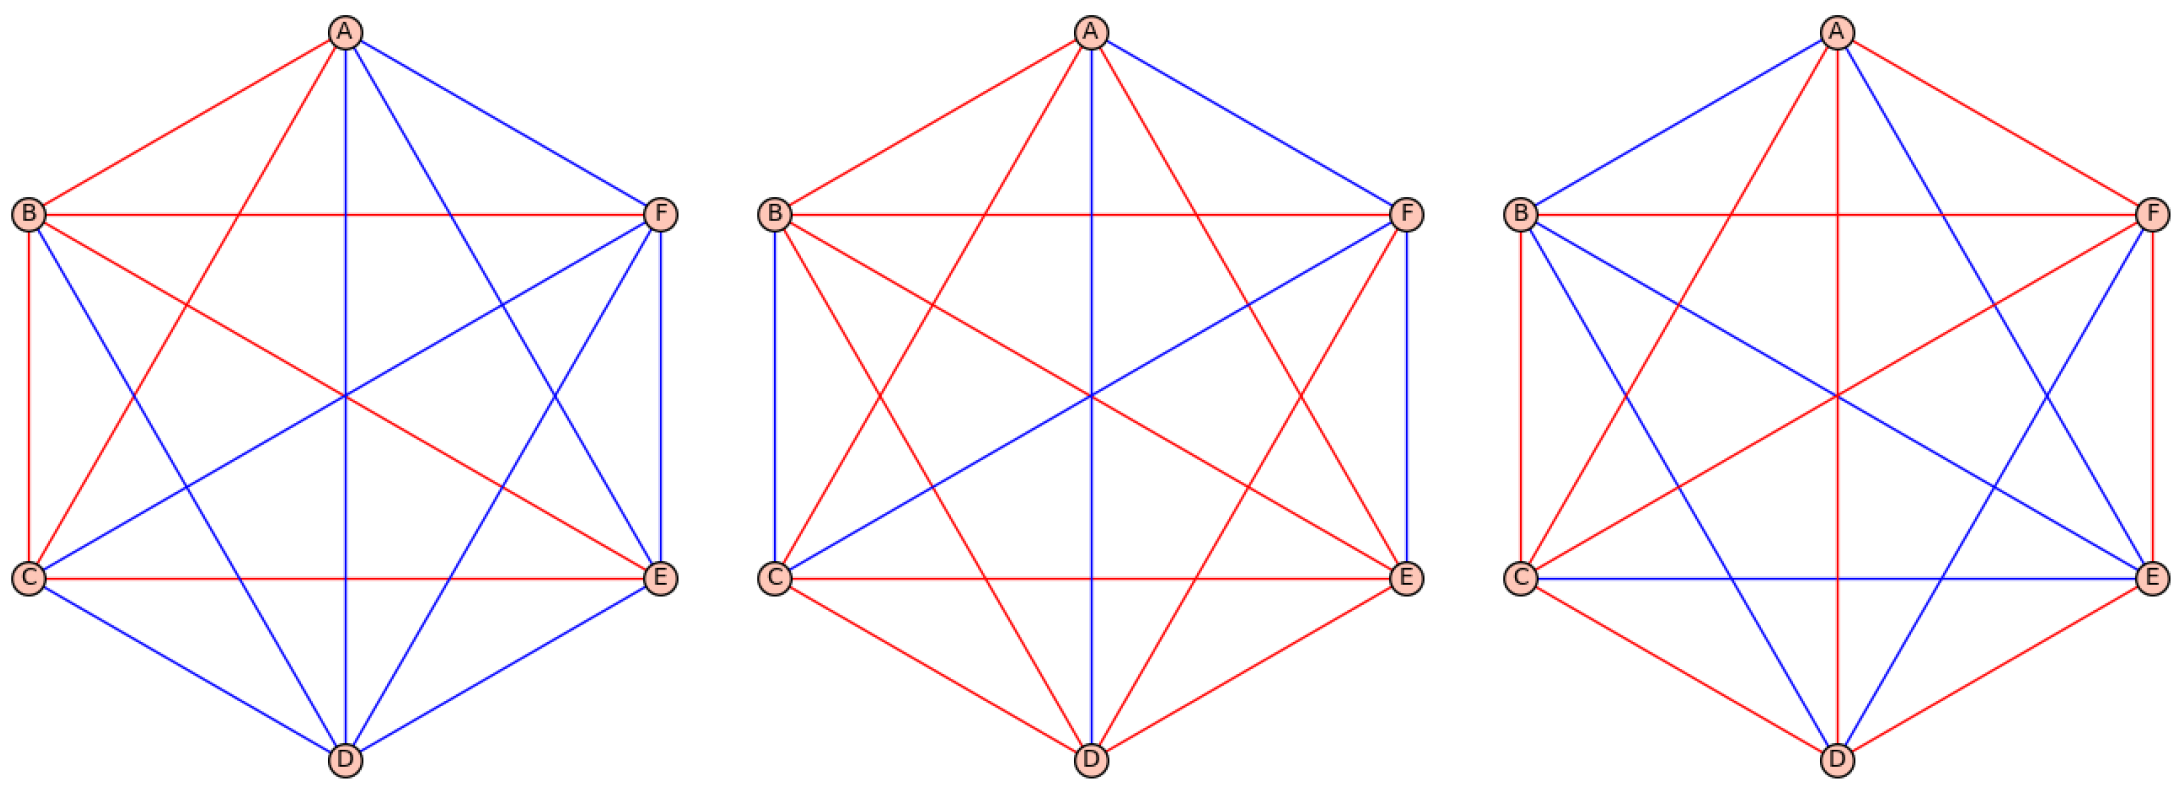
\includegraphics[width=0.9\linewidth]{Images/Figure10.png}
    \caption{3 randomly colored examples, each of which has either a red triangle or a blue triangle.}
    \label{f:10}
\end{figure}
\begin{remark}
\cref{f:10} makes it clear that in some sense we are looking for appearance of a uniformly colored triangle sitting inside the (bigger) graph. Ramsey theory, a branch in the field of combinatorics, focuses precisely on questions of these kind.
\end{remark}
\begin{comment}
\[
	\sum_{v\in V}degree(v) = 2|E|
.\] 
Introduce Ramsey's theorem
\end{comment}
We conclude this section by stating two definitions which will turn out to be useful in the upcoming sections.
\begin{definition}[$k$-Permutation]
A $k$-permutation on $[n]=\{1,2,\cdots,n\}$ is a bijection between two $k$-element subsets of $[n]$. 
\end{definition}
\begin{definition}[Circular $k$-Permutation]
	$k$-permutations  $\pi$ and $\sigma$ are called circular equivalents if there exists a shift  $s\in [k]$ such that  $i+s\equiv j(\text{mod} \ k)$.
\end{definition}
\section{The Principle of Inclusion-Exclusion}
\textcolor{red}{
[This section is a work in progress!!!] Note to scribe:
\begin{enumerate}
    \item Finish the proof of Theorem 4.2
    \item Rewrite the proof of Claim 4.1
    \item Write and prove Claim 4.2
\end{enumerate}
}
Recall that for finite sets $A$ and $B$, the cardinality of their union is given by $|A \cup B| = |A| + |B| - |A \cap B|
$. This formula, which adds (includes) the sizes of $A$ and $B$ while subtracting (excluding) the overcount in $|A \cap B|$ encapsulates the essence of the inclusion-exclusion principle. We start with a useful generalization of the motivating formula we just discussed.
\begin{theorem}[Inclusion-Exclusion Principle]
	Given finite sets $A_{1},\cdots,A_{k}$, 
	\[
		|\bigcup_{i=1}^k A_i| = \sum_{n=1}^{k}\left(-1  \right)^{n+1}\left( \sum_{1\leq i_{1}<\ldots<i_{n}\leq k+1}|A_{i_{1}}\cap \cdots A_{i_{n}}| \right) 
	.\] 
 \label{t:4.1}
\end{theorem}
To see how useful this result is, we state two examples.
\begin{question}
How many of the first $1000$ natural numbers are not divisible by $2,3$ or $6$? \label{q:4.1}
\end{question}
\begin{solution}
Out of the first $1000$ natural numbers, notice how, there are $\left \lfloor{1000/n}\right \rfloor$ numbers which are divisible by $n$. Now, by the inclusion exclusion principle we have 
\[
1000-500-333-200+\left \lfloor{1000/6}\right \rfloor+\left \lfloor{1000/15}\right \rfloor+\left \lfloor{1000/10}\right \rfloor-\left \lfloor{1000/30}\right \rfloor=266
\]
natural numbers which are not divisible by $2,3$ or $6$. 
\end{solution}
\cref{q:4.1} motivates an equivalent version of \cref{t:4.1} which we shall now state and prove.
\begin{theorem}[Inclusion-Exclusion Principle]
For $1\leq i\leq$, let $A_i$ be subsets of a set $X$. Then the number of elements of $X$ which do not lie in any of the $A_i$s is given by
\[
\sum_{I\subseteq \{1,\cdots,n\}}(-1)^{|I|}|A_I|
\] where $A_I = A_{i_1}\cap A_{i_2}\cap \cdots \cap A_{i_k}$ for $I=\{i_1,\cdots,i_k\}$. 
\label{t:4.2}
\end{theorem}
\begin{proof}
\end{proof}
\begin{comment}
\begin{proof}
Notice how for every $x\in X$ one of the following is true.
\begin{enumerate}
    \item $x\not\in A_i$ for all $i$
    \item $x\in A_i$ for some $i$, i.e, for some $I$ we have $x\in A_I = A_{i_1}\cap A_{i_2}\cap \cdots \cap A_{i_k}$. Since the said $I$ can be chosen in $\binom{n}{k}$ ways. 
\end{enumerate}
\end{proof}    
\end{comment}
Now we state a corollary of \cref{t:4.2}.
\begin{claim}
The number of surjective mappings from $[n]=\{1,2,3,\cdots,n\}$ to $[k]=\{1,2,3,\cdots,k\}$ is given by \[
    \sum_{i=0}^{k}(-1)^i\binom{k}{i}(k-i)^n
    \]
\end{claim}
\begin{proof}
We mimic the setting of \cref{t:4.2}. Choose $X$ to be the set of all mappings from $[n]$ to $[k]$, and $A_i$ to be the set of all maps from $[n]$ to $[k]$ such that $i$ is not in the range. Notice how $|X|=k^n$, $|A_i|=(k-1)^n$, and $|A_I| = |A_{i_1}\cap A_{i_2}\cap \cdots \cap A_{i_j}|=(k-j)^n$. Now the claim follows. 
\end{proof}
\begin{comment}
    Explain the cardinalities of $A_i$ and $X$ better.
\end{comment}
\begin{remark}
Since every surjection from $[n]$ to $[n]$ is necessarily a bijection, and by \cref{q:1.5} we know that there are $n!$ bijections from $[n]$ to $[n]$, we've proved a combinatorial identity, namely that
\[
\sum_{i=0}^{n}\binom{n}{i}(n-i)^n=n!.
\]
\end{remark}
We now give an application of the inclusion-exclusion principle in number theory. More specifically, consider the Euler's $\varphi$ function which is defined as
\begin{align*}
    \varphi: &\mathbb{N}\to \mathbb{N} \\
    &n\rightsquigarrow |\{x\in\mathbb{N}: x< n, \text{gcd}(x,n)=1\}|.
\end{align*}
For instance, $\varphi(1)=|\{1\}|=1$, $\varphi(2)=|\{1\}|=1$, $\varphi(3)=|\{1,2\}|=3$, and so on. In essence, $\varphi(n)$ counts the positive integers which are less $n$ and are co-prime to $n$. It is clear that for a prime $p$, $\varphi(p) = p-1$. More generally for a natural number $r>0$ we also have
\[
\varphi(p^r) = p^r-\left\lfloor \dfrac{p^r}{p}\right\rfloor = p^r-p^{r-1}.
\]
\begin{comment}
State the fundamental theorem of arithmetic. 
\end{comment}

\begin{theorem}
For $n=p_1^{a_1}\cdots p_k^{a_k}$ we have 
\begin{align*}
\varphi(n) &= n\left(1-\dfrac{1}{p_1}\right)\cdots\left(1-\dfrac{1}{p_k}\right) \\
\end{align*}
\end{theorem}
\begin{proof}
We are interested in counting all the numbers $a$ in the set $[n]=\{1,2,3,\cdots,n\}$ is relatively prime to $n$. This happens if and only if $a$ is not divisible by any of the primes $p_1,\cdots,p_k$. Now, let $A_i$ be the subset of $[n]$ that contains all numbers which are divisible $p_i$. By our setup it is clear that 
\begin{align*}
\varphi(n) &= |[n]\backslash \bigcup_{i=1}^{n}A_i| \\
&= n - |\bigcup_{i=1}^{n}A_i| \\
&= n - \sum_{I_{\neq \emptyset}\subseteq [m]}(-1)^{|I|+1}|\bigcap_{i\in I}A_i| \quad \text{(By \cref{t:4.2})}
\end{align*}
Notice how $\cap_{i\in I}A_i$ contains elements of $[n]$ which are not divisible by any $p_i$ where $i\in I$, and hence also not divisible by $\prod_{i\in I}p_i$. It follows that
\begin{align*}
&|\cap_{i\in I}A_i| = \dfrac{n}{\prod_{i\in I}p_i} \\
&\implies \varphi(n) = n - \sum_{I_{\neq \emptyset}\subseteq [m]}(-1)^{|I|+1}\dfrac{n}{\prod_{i\in I}p_i} \\
&\implies \varphi(n) = n\left(1+\sum_{I_{\neq\emptyset}\subseteq [m]}(-1)^{|I|}\dfrac{1}{\prod_{i\in I}p_i}\right) \\
&\implies \varphi(n) = n\left(1+\sum_{I_{\neq\emptyset}\subseteq [m]}\prod_{i\in I}\dfrac{-1}{p_i}\right) \\
&\implies \varphi(n) = n\prod_{i=1}^{m}\left(1-\dfrac{1}{p_i}\right)
\end{align*}
\begin{comment}
Fill the details in the proof out.
\end{comment}
\end{proof}
Now that we have counted the number of elements which are co-prime to $n$, we are interested in finding their sum. In this spirit consider the following claim.
\begin{claim}
\end{claim}
We conclude this section by introducing derangements. 
\begin{question}
Suppose $n$ people go a party and each person is wearing a different hat. In how many ways can the $n$ people return from the party such that nobody is wearing their original hat?    
\end{question}
\begin{solution}
It is clear that we are counting the number of permutations on $[n]$ with no fixed points. Let $A_j$ be the set of permutations which consist of all permutations such that $j$ is fixed point. Now the inclusion-exclusion principle the number of permutations with no fixed points are
\begin{align*}
D_n:=|\underbrace{A_1^c}_{1 \text{ is not fixed}} \cup \underbrace{A_2^c}_{2 \text{ is not fixed}} \cup \underbrace{A_3^c}_{3 \text{ is not fixed}} \cup \quad \cdots \quad \underbrace{\cup A_n^c}_{n \text{ is not fixed}}|.
\end{align*}
Since it is clear that $|A_j|=(n-1)!$, we have
\[
|A_{i_1}\cup A_{i_2}\cup \cdots \cup A_{i_k}| = (n-k)!.
\]
Once again by the inclusion-exclusion principle
\begin{align*}
    D_n &= n! - \binom{n}{1}(n-1)! + \binom{n}{2}(n-2)! -  \cdots + (-1)^n\binom{n}{n}0! \\
    &= n! - \dfrac{n!}{1!} + \dfrac{n!}{2!} - \cdots + (-1)^n\dfrac{n!}{n!}
\end{align*}
\end{solution}

